	\section*{Exercice 3 (5 points)}
	

	
	\subsection*{1. Représenter la situation par un arbre pondéré.}
	
\begin{center}
	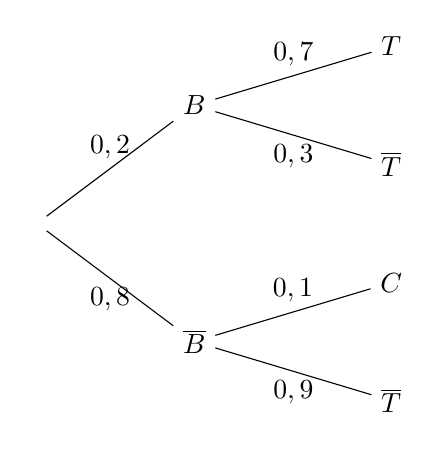
\begin{tikzpicture}
		[level 1/.style={level distance=2cm,
			sibling distance=3cm},
		level 2/.style={level distance=2.5cm,
			sibling distance=1.5cm}]
		\node {} [grow'=right]
		child {node {$B$}
			child {node {$T$}
				edge from parent node[above] {$0,7$}
			}
			child {node {$\overline T$}
				edge from parent node[below] {$0,3$}
			}
			edge from parent node[above] {$0,2$}
		}
		child {node {$\overline B$}
			child {node {$C$}
				edge from parent node[above] {$0,1$}
			}
			child {node {$\overline T$}
				edge from parent node[below] {$0,9$}
			}
			edge from parent node[below] {$0,8$}
		}
		;
	\end{tikzpicture}
\end{center}
	
	\subsection*{2. Quelle est la probabilité que l’angine soit bactérienne et que le test soit positif ?}
	
	On a $P(B \cap T) = P(B) \times P_B(T) = 0,2 \times 0,7 = 0,14$.
	
	\subsection*{3. Montrer que la probabilité que le test soit positif est 0,22.}
	
	D’après la loi des probabilités totales :
	\[
	P(T) = P(T \cap B) + P(T \cap \overline{B}) = 0,14 + 0,8 \times 0,1 = 0,14 + 0,08 = 0,22
	\]
	
	\subsection*{4. Un malade est choisi au hasard parmi ceux dont le test est positif. Quelle est la probabilité pour que son angine soit bactérienne ?}
	
	Il faut calculer $P_T(B) = \dfrac{P(T \cap B)}{P(T)} = \dfrac{0,14}{0,22} = \dfrac{14}{22} = \dfrac{7}{11} \approx 0,636$.\\ La probabilité est donc environ 0,636.
	
